\chapter{Deep Q-Learning}
\lecture{Feb. 23}
Similar to homework questions. Some proof, think-through questions. Mix of intuition, understanding,
and some mathematical details. Typically one challenging question at the end of the exam. Up to and including Deep Q-Learning.

\section{Experience Relay}
Put all data in a buffer and randomly sample.

\section{Target Network}
Q-learning gradient update:
\[
  w = w + \alpha(r_k + \gamma \max_{b} Q(w)(s_{k+1}, b) - Q(w)(s_k, a_k)) \nabla_{w} Q(w)(s_k, a_k)
\]
In supervised learning, the target does not depend on the parameter. In Q-learning, target $r_k + \gamma \max_{b} Q(w)(s_{k+1}, b)$ depends on $w$, so the target is moving as the parameter is updated.
\section{DQN Algorithm}
\section{Maximization Bias in Q-Learning}
Let $\hat{\pi} = \arg \max_{a} \hat{Q}(s,a)$ and $\hat{V}_{\hat{\pi}} = \max_{a} \hat{Q}(s,a)$.
\[
  \E[\hat{V}_{\hat{\pi}}] = \E[\max_{a} \hat{Q}(s,a)] \geq \max_{a} \E[\hat{Q}(s,a)]
\]
The greedy policy obtained from the estimated $Q$ values can yield a maximization bias when the number of samples are finite. Maximization bias is DQN, from [Van Hasselt et al., 2016].

\section{Double Estimator}
Consider two random variables $Y^1$ and $Y^2$ with mean values $\mu^1$ and $\mu^2$. Let $\Yc^1$ and $\Yc^2$ be the sets of i.i.d. samples of $Y^1$ and $Y^2$. Our goal is to esimate $\max_{i} \mu^i$. With a single estimator, we let $\hat{\mu}^i = \frac{1}{|\Yc^i|} \sum_{y\in\Yc^i} y$ and let $\hat{i}^* = \arg\max_{i} \hat{\mu}^i$. Then, single esitmator is $\hat{\mu}_\text{max} = \hat{\mu}^{\hat{i}^*}$. This single estimator gives an overestimate because we are using the same samples both to determine the maximizer and value. \\

\noindent Possible solution is to divide the samples into two sets and use them to learn two independent estmates. Now we split $\Yc^i$ into $\Yc_{A}^i$ and $\Yc_{B}^i$ and then compute $\hat{\mu}_{A}^i = \frac{1}{|\Yc_{A}^i|} \sum_{y\in\Yc_{A}^i} y$ and $\hat{\mu}_{B}^i = \frac{1}{|\Yc_{B}^i|} \sum_{y\in\Yc_{B}^i} y$. Now find $\hat{i}^* = \arg\max_{i}\hat{\mu}_{A}$ and get double estimator $\hat{\mu}_\text{max} = \hat{\mu}_B^{\hat{i}^*}$. We can show that the double estimator is an underestimator, i.e., $\E[\hat{\mu}_{\text{max}}] \leq \max_{i} \E[Y^i]$.
\begin{proof}
  Let $i^* = \arg\max_{i} \E[Y^i]$ be the true maximizer. Then,
  \begin{align*}
    \E[\hat{\mu}_{\text{max}}] & = \E[\hat{\mu}_B^{\hat{i}^*}] = \P(\hat{i}^* = i^*) \E[\hat{\mu}_{B}^{\hat{i}^*} \mid \hat{i}^* = i^*] + \P(\hat{i}^* \neq i^*) \E[\hat{\mu}_{B}^{\hat{i}^*} \mid \hat{i}^* \neq i^*] \\
                               & = \P(\hat{i}^* = i^*) \max_{i} \E[Y^i] + \P(\hat{i}^* \neq i^*) \E[\hat{\mu}_{B}^{\hat{i}^*} \mid \hat{i}^* \neq i^*]                                                                 \\
                               & \leq \P(\hat{i}^* = i^*) \max_{i} \E[Y^i] + \P(\hat{i}^* \neq i^*) \max_{i} \E[Y^i] = \max_{i} \E[Y^i]
  \end{align*}
\end{proof}
\section{Double DQN}
Use one Q-network to select the max-action and another Q-network to evaluate it. DQN maintains two networks anyway (one as the target
network and one as the current network)
\[
  w = w + \alpha(R + \gamma \max_{b}Q(w^-)(s^{\prime}, b) - Q(w)(s,a)) \nabla Q(w)(s,a)
\]
where $w^- = w$, after every $N$ steps. To implment double DQN, use the current Q-network to select the max-action, and the target
Q-network to evaluate that action
\[
  w = w + \alpha(r + \gamma Q(w^-)(s^{\prime}, \arg\max_{b} Q(w)(s^{\prime}, b)) - Q(w)(s,a)) \nabla Q(w)(s,a)
\]

\subsection{Advantage Function}
The advantage function is defined as
\[
  A_\pi (x,a) = Q_\pi (x,a) - V_\pi(x)
\]
The value function measures how good it is to be in a particular state; the Q function measures the value of choosing particular action when in that state; the advantage function obtains a relative measure of the importance of each action.
\subsection{Dueling DQN Architecture}
In DQN, there is a single stream to estimate Q function. In DDQN, two streams separately estimate (scalar) state-value and the advantages for each action. These two streams are particularly useful in states where its actions do not affect the environment in any relevant way.
Dueling architecture can more quickly idenitify the correct action during policy evaluation as redundant or similar actions are added to the learning problem.

\subsection{Prioritized Experience Replay (sampling from Replay Buffer)}
Some experience (data samples $(s_i, a_i, r_i, s_{i+1})$) may be more informative than other. In experience relay, samples are taken uniformly at random from the replay buffer. Uniform sampling will not be able to make use of such informative samples efficiently. \\

\noindent Can we prioritize the samples to accelerate the learning progress? Intuition: prioritize a sample based on how much we can learn from a transition (expected learning progress). Proxy for this is TD error: for $e_i = (s_i, a_i, r_i, s_{i+1})$, TD error is defined as
\[
  \delta_i = r_i + \gamma \max_{b}Q(w)(s_{i+1}, b) - Q(w)(s_i, a_i)
\]
In prioritized experience replay, sample $e_i$ is selected with probability $p_i$,
\begin{enumerate}[label=\textbf{--}, topsep=5pt, itemsep=-5pt]
  \item Proportional sampling: $p_i = \frac{|\delta_i|^c}{\sum_{i}|\delta_i|^c}$
  \item Rank-based sampling: $p_i = \frac{1}{\rank(e_i)}$ \\
        where the rank of $e_i$ when the repla memory is sorted according to $|\delta_i|$.
\end{enumerate}
Priorities experience replay offers a performance improvement over DQN.
\subsection{Rainbow DQN}
The deep reinformcent learning community has made several independent improvements to the DQN
algorithm. However, it is unclear which of these extensions are complementary and can be fruitfully combined.
Hessel et al., 2018,  shows that the combination provides state-of-the-art performance on the Atari 2600 benchmark, both in terms of data efficiency and final performance.
% {https://arxiv.org/abs/1710.02298}

\begin{figure}[h!]
  \centering
  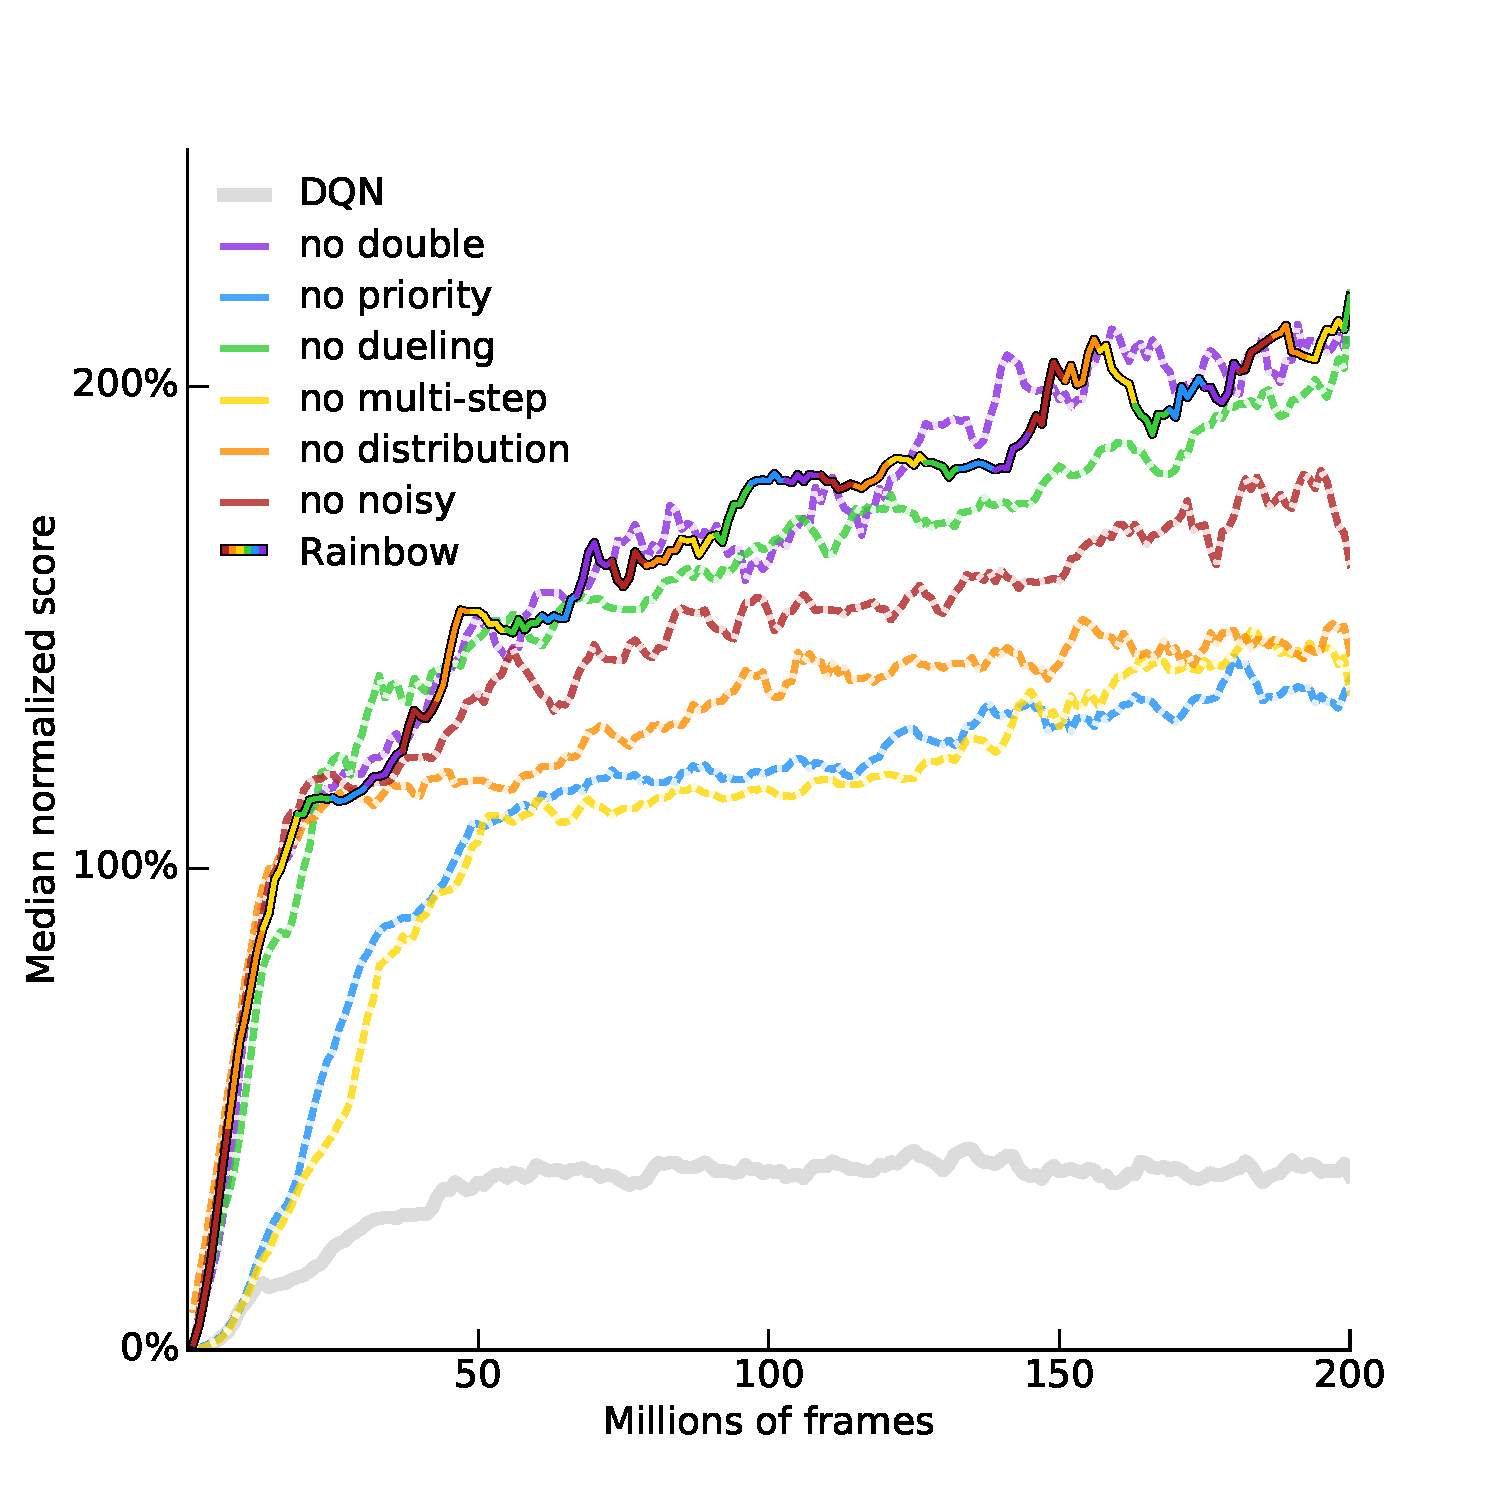
\includegraphics[width=0.4\textwidth]{figures/Plots_SecondPlot.pdf}
  \vspace*{-0.2in}
  \caption{Median human-normalized performance}
\end{figure}

\noindent Later on, Agent57 was the first deep reinformcent learning agent to obtain a score that is above the human
baseline on all 57 Atari 2600 games.

% L09 end 
